\documentclass[12pt]{article}
\usepackage[hcentering,bindingoffset=20mm]{geometry}
\usepackage{placeins}
\usepackage[numbib]{tocbibind}
\usepackage{rotating}
\usepackage[square,sort,comma,numbers]{natbib}
\usepackage{graphicx}
\usepackage{tabularx}
\linespread{1.3}
\usepackage{gensymb}
\usepackage{longtable}
\usepackage{lscape}
\usepackage{url}
\addtolength{\textwidth}{2cm}
\addtolength{\hoffset}{-1cm}
\addtolength{\textheight}{2cm}
\addtolength{\voffset}{-1cm}
\setlength{\parindent}{0pt}
\title{Development of semi-quantitative PCR assays for the detection and enumeration of ciguatoxin producing \emph{Gambierdiscus lapillus} and \emph{Gambierdiscus polynesiensis} (Gonyaulacales, Dinophyceaes).}
\author{}
\date{}
\begin{document}
\maketitle

%\begin{figure} 
%\includegraphics[scale=0.65]{CFP_diagram.png} 
%\caption{The mechanism of bioaccumulation of ciguatoxins, with \emph{G. polynesiensis} at the base of the food web inhabiting macroalgae, e.g. a \emph{Padina} spp. \cite{padina}. A herbivore, e.g. white trevally (\emph{Pseudocaranx dentex}) \cite{trevally} consumes CTX from \emph{G. polynesiensis} along with the macroalgae, which is then either passes directly to humans through consumption, or through an intermediary piscivorous vector such as Australian spotted mackerel (\emph{Scomberomorus munroi}) \cite{mackerel}. Image of \emph{G. polynesiensis} (strain CG15) taken by A. L. Kretzschmar, 2016, Nikon Eclipse TS100 equipped with an Infinite Luminera 1 camera.} 
%\label{fig:bioacc}
%\end{figure} 
%\FloatBarrier

\begin{figure} 
%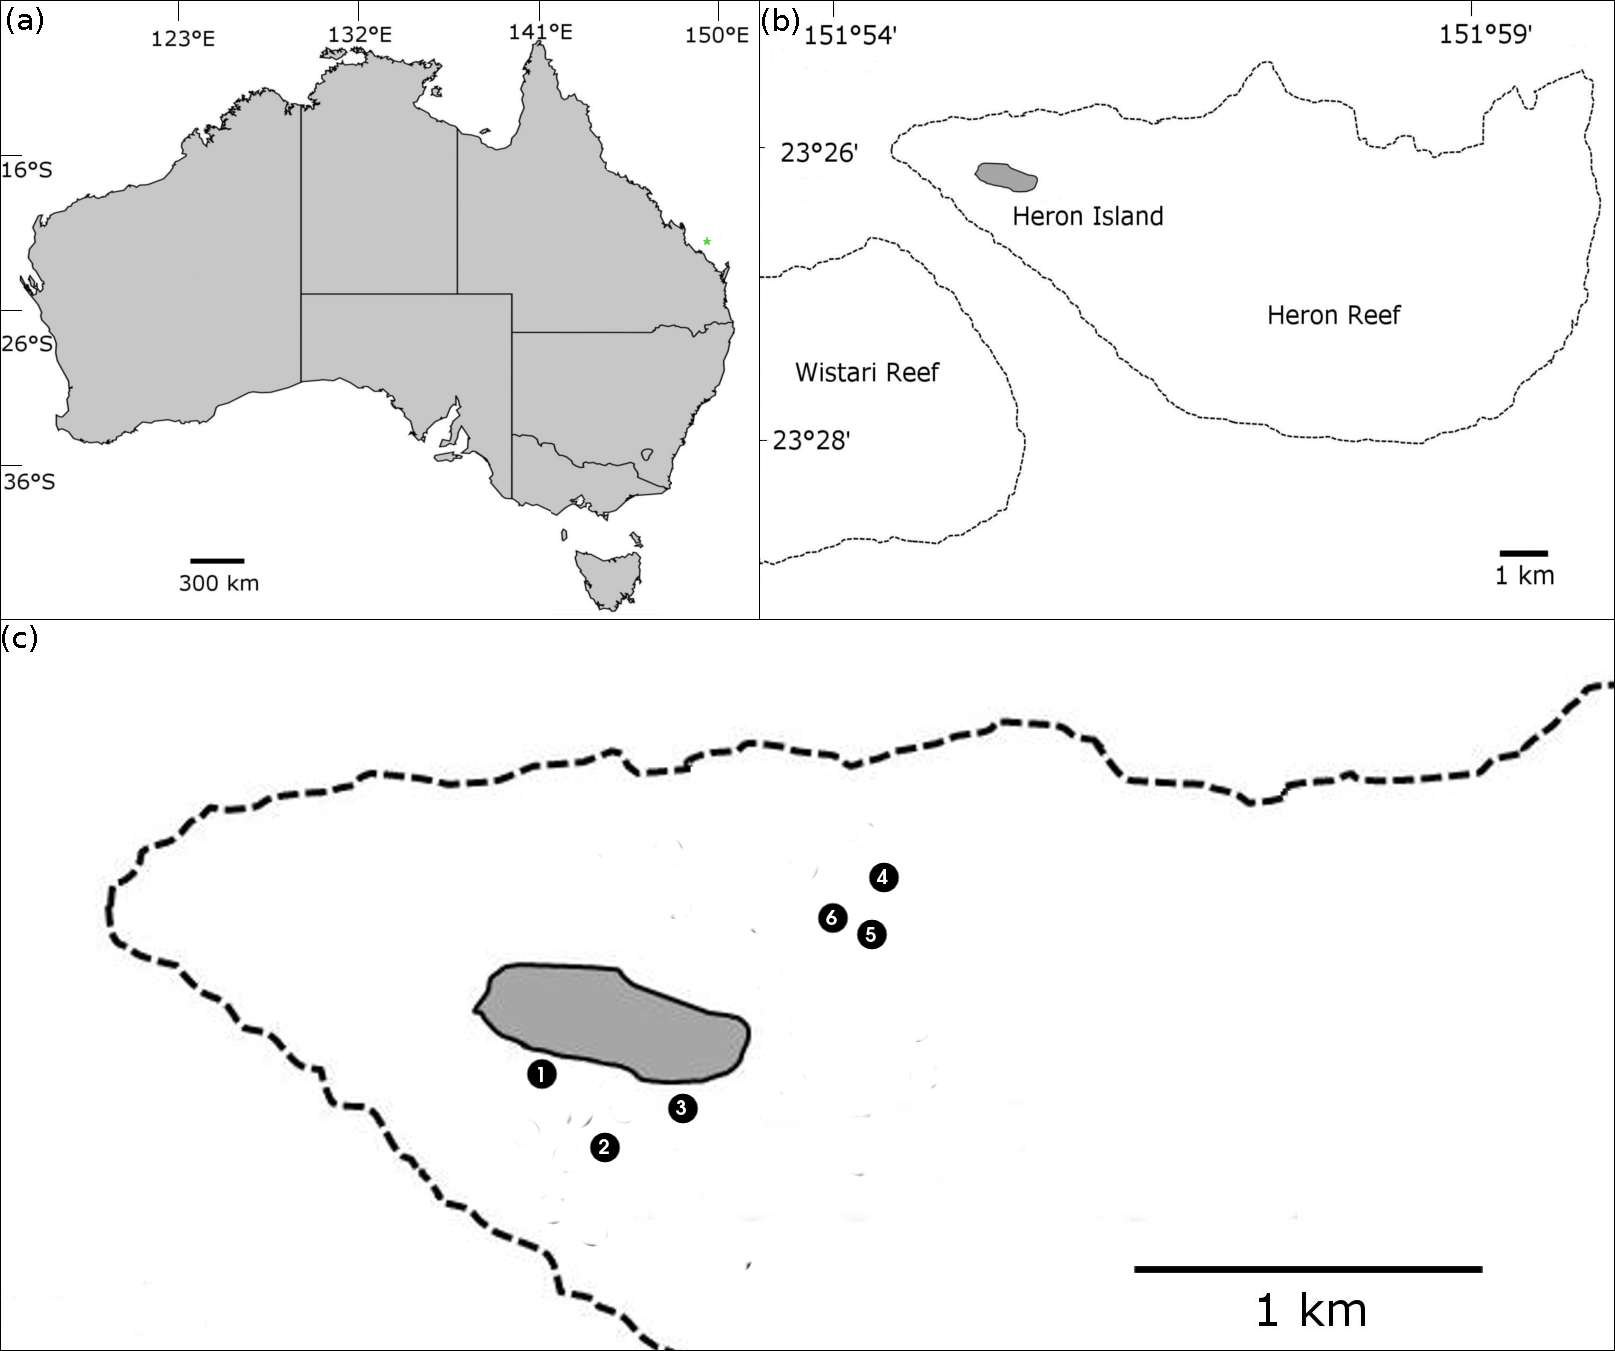
\includegraphics[scale=1.5]{Hero_qpcr-figs/Fig1_Heron_sample-map_May18.png} 
\caption{(A) Map of Australia, with the position of Heron Island (grey circle); (B) Heron Island including surrounding reefs; (C) Sampling sites around Heron Island.} 
\label{fig:samplesites}
\end{figure} 
\FloatBarrier

\begin{figure}
%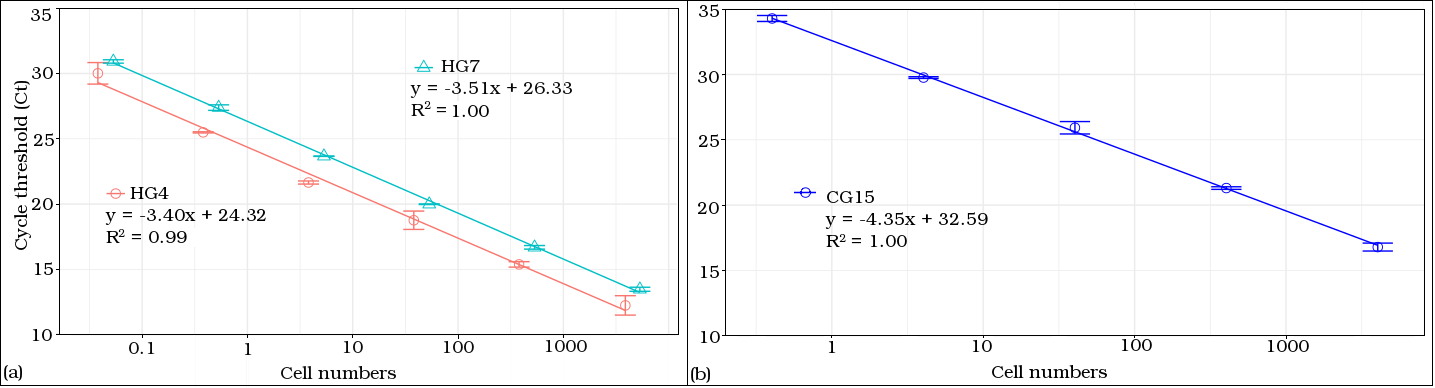
\includegraphics[scale=.4]{Hero_qpcr-figs/Fig2_cell-based-stds-merged.png}
\caption{qPCR cell based standard curves of (A) \emph{G. lapillus} strains HG4 (circle) and HG7 (triangle); and (B) \emph{G. polynesiensis} strains CG14 and CG15.} %Error bars represent the deviation of technical replicates during reactions.}
\label{fig:stdCurve}
\end{figure}
\FloatBarrier

\begin{figure}
%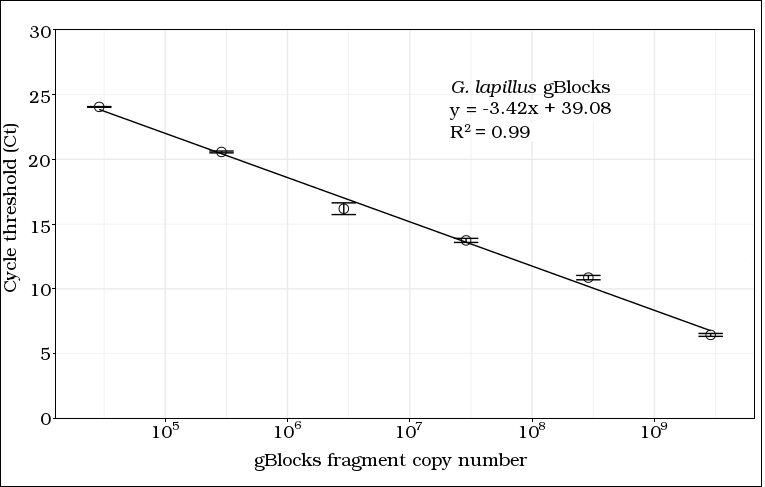
\includegraphics[scale=.4]{Hero_qpcr-figs/Fig3_gblocks-standards.png}
\caption{qPCR gene based standard curves of (A) \emph{G. lapillus} and (B) \emph{G. polynesiensis}.} %Error bars represent the deviation of technical replicates during reactions.}
\label{fig:lapigblocks}
\end{figure}
\FloatBarrier

\FloatBarrier 
\begin{figure} 
%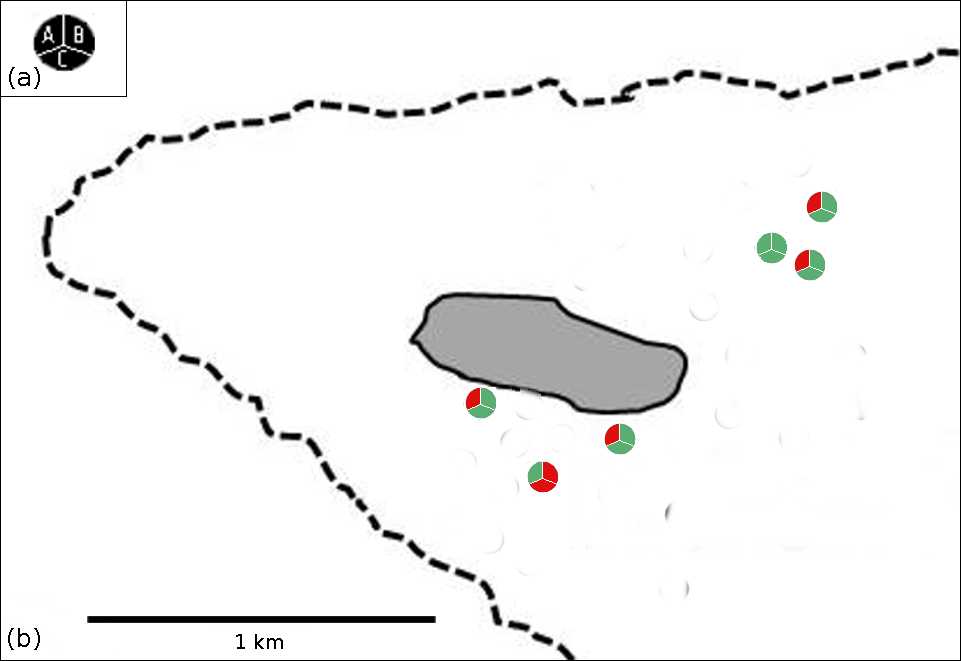
\includegraphics[scale=2]{Hero_qpcr-figs/Fig4_Heron-positive-negative-samplingsites_May18.png} 
\caption{\emph{G. lapillus} presence at the sampling sites around Heron Island. The spatial replicates for each site are set up as shown in (A); the sites in (B) linked to numbering in Fig. ~\ref{fig:samplesites} where positive (green) and negative (red) as per Supplementary Table 1.} 
\label{fig:envposneg}
\end{figure} 
\FloatBarrier

\FloatBarrier 
\begin{figure} 
%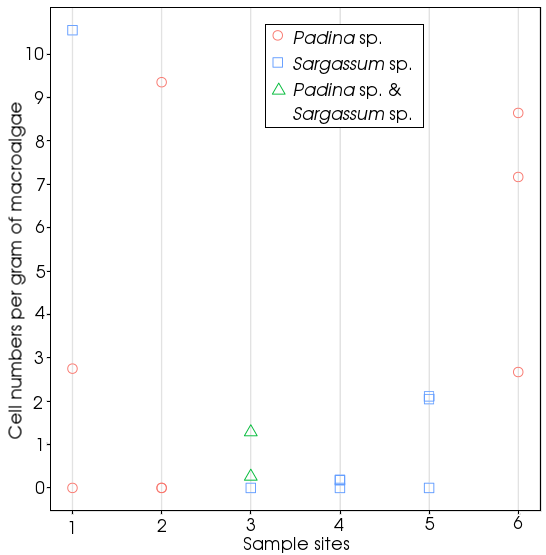
\includegraphics[scale=.7]{Hero_qpcr-figs/Fig5_Env-sites-May18.png} 
\caption{Detection of \emph{G. lapillus} per spatial replicate at each sampling site, cell numbers as normalised to HG7 standard curve (Fig. ~\ref{fig:stdCurve}A). Spatial replicates cper macroalgal substrate where \emph{Sargassum} sp. are squares, \emph{Padina} sp. are circles and mixed macroalgal substrates are triangles (see Supplementary Table 1.).} 
\label{fig:envHG7}
\end{figure} 
\FloatBarrier



\newpage
\bibliographystyle{acm}
\bibliography{references.bib}
\end{document}